\documentclass[letterpaper,10pt]{article}
%paquetes
\usepackage[spanish, es-noquoting]{babel}%formato de las tablas
\usepackage[utf8]{inputenc}
\usepackage{enumerate}
\usepackage{graphicx}
\usepackage{float}
\usepackage[T3,T1]{fontenc}
\usepackage{amsmath,wasysym,amssymb,amsfonts,textcomp,latexsym}
\usepackage{hyperref}
\usepackage{appendix}
\usepackage{enumitem}
\usepackage[ruled,vlined,lined,linesnumbered,algosection,spanish]{algorithm2e}
\usepackage{multimedia}
%\usepackage[intlimits]{amsmath}
\usepackage{flexisym}
\usepackage{xparse}
\usepackage{mathtools}
\usepackage{bm}
%\usepackage{draftwatermark}

%\SetWatermarkText{\textsc{Borrador}}
%\SetWatermarkScale{5}
%\SetWatermarkAngle{55}
%%%
% \usepackage{ragged2e}
% \usepackage{pstricks,enumerate}

%\setpapersize{A4}
% Numeración
%\usepackage{vmargin}
%\setmargins{1.5cm}       % margen izquierdo
%{1.5cm}                        % margen superior
%{16.5cm}                      % anchura del texto
%{23.42cm}                    % altura del texto
%{10pt}                           % altura de los encabezados
%{1cm}                           % espacio entre el texto y los encabezados
%{0pt}                             % altura del pie de página
%{2cm}                           % espacio entre el texto y el pie de página
\setcounter{secnumdepth}{30}
\title{Propuesta Alberto Rodríguez Sánchez}

\begin{document}
\renewcommand{\refname}{Bibliografía}.
% Página sin estilo para portada quitar encabezado, pie y número de página
\thispagestyle{empty}

\begin{center}
    {\Huge Universidad Autónoma Metropolitana }\\
    {\huge Unidad Azcapotzalco}\\
    \vspace{0.5cm}
    {\Large División de Ciencias Básicas e Ingeniería}\\
    \vspace{1.0cm}
    {\large Posgrado en Optimización}\\
    \vspace{2.0cm}    
    {\Large Preservación de la Diversidad y Manejo de los Puntos de Referencia en Algoritmos Evolutivos Multiobjetivo}\\
    % 
    %
    \vspace{1.0cm}
    {\large Propuesta de Proyecto de Investigación}\\
    \vspace{2.0cm}
    {\large\textbf{Alumno:}}\\
    Alberto Rodríguez Sánchez\\
    %\bigskip 2153800510\\
    \vspace{1.5cm}
    \bigskip
    {\large\textbf{Asesores:}}\\
    Dr. Antonin Ponsich\\
    
    \vspace{1.5cm}
     2017\\
    \vspace{1.0cm}
    Ciudad de México\\
\end{center}
\newpage
\tableofcontents
\newpage
\section{Introducción}

Los problemas de optimización multiobjetivo \textbf{(MOP)} ha sido de gran interés en la comunidad científica e industrial, ya que son comunes aquellos problemas que requieren
considerar múltiples objetivos, incluyendo tiempo, costos, cantidad, calidad, etc. Estos objetivos se encuentran típicamente en conflicto y se pueden encontrar inmersos en
diferentes problemas como: ruteo de vehículos, localización, cadenas de suministro, calendarización, entre otros.\\

Esta clase de problemas ha sido tradicionalmente atacada reduciendo el \textbf{MOP} en un problema mono-objetivo (estrategias de suma agregativa ponderada, de restricciones-$\epsilon$,
de programación por metas), desde los años 1990, los esfuerzos de investigación se han dedicado al desarrollo de técnicas metaheurísticas, y particularmente Algoritmos Evolutivos (AEs).
Desde el punto vista metaheurístico, se han generado tres grandes enfoques para resolver \emph{MOP}:

\begin{itemize}
 \item Basado en descomposición
 \item Basado en dominancia
 \item Basado en métricas
\end{itemize}

El enfoque de descomposición explícitamente descompone un problema multiobjetivo en $N$ problemas de optimización escalar y suele introducir técnicas poblacionales para
la resolución simultánea de ellos. Bajo este enfoque, es importante seleccionar los problemas escalares conforme a algún criterio que permita mejorar la diversidad del conjunto
de soluciones arrojado, dejando la convergencia al submétodo de resolución. Un marco de trabajo moderno con este enfoque es el algoritmo evolutivo multiobjetivo basado en
descomposición (\emph{MOEA/D})\cite{4358754}.
\newline

En el enfoque de dominancia, se utiliza la relación de dominancia para inducir un orden parcial en el espacio de los objetivos y, de esta manera, decidir cuándo una solución
en dicho espacio es comparable con otra y, en este caso, cuál es la mejor. Cabe mencionar que dicho orden parcial está limitado en espacios de altas dimensiones puesto que una gran
cantidad de soluciones serán no comparables, mermando en consecuencia la efectividad de los procedimientos de selección. El algoritmo genético de ordenamiento no dominado
(\emph{NSGA-III})\cite{6600851} es un marco de trabajo moderno con esta estrategia, que incorpora además técnicas de nichos para mantener la diversidad.
\newline

Finalmente, el enfoque basado en métricas convierte el problema multiobjetivo original en un problema mono o multiobjetivo diferente que optimiza el valor de métricas de desempeño,
representando la calidad del conjunto de soluciones obtenidas tanto en términos de convergencia como de dispersión y uniformidad de su distribución. Una métrica popular
es el hipervolumen ya que es la única acorde a la definición de  optimalidad de Pareto (i.e., las soluciones Pareto-óptimas son aquellas que maximizan el hipervolumen).
Sin embargo, calcular el hipervolumen se vuelve costoso conforme aumenta la dimensión del problema multiobjetivo original, por ejemplo, la mejor forma conocida de calcular
el hipervolumen tiene una complejidad de $O(n^2m^3)$ donde $n$ es el número de soluciones aproximadas y $m$ el número de objetivos.
\newline

Un conjunto de soluciones candidatas entregadas por cualquiera de los enfoques antes mencionados debe de cumplir con criterios de convergencia y diversidad para ser
considerado aceptable. Esta meta de obtener un conjunto de soluciones diversas y uniformemente distribuidas se ve dificultada cuando los métodos de solución deben lidiar con:

\begin{itemize}
 \item Convexidad o no convexidad del frente óptimo de Pareto.
 \item Discontinuidad del frente óptimo de Pareto.
 \item Densidad no uniforme de las soluciones en el frente óptimo de pareto.
\end{itemize}

En general, los enfoques basados en dominancia y descomposición utilizan puntos y/o vectores de referencia, que representan direcciones de búsqueda en el espacio objetivo. Pero si bien se han estudiado distintos métodos para generarlos,
sus valores se mantienen clásicamente fijos durante el transcurso de la ejecución del algoritmo. Esta estrategia puntos/vectores de referencia estáticos experimenta justamente problemas cuando el frente óptimo presenta las fuentes de dificultad antes mencionadas (no-convexidad, degeneración, discontinuidad del frente óptimo).
Por lo tanto, el presente proyecto se propone, en primer lugar, comparar la eficacia de diferentes métodos de generación de dichos puntos/vectores de referencia;
y posteriormente, investigar técnicas que permitan ajustarlos en el transcurso de la búsqueda, con el fin de mejorar la diversidad del conjunto solución final.\\

El resto de la presente propuesta se organiza de la siguiente manera. En una segunda sección, se plantea el problema de optimización multiobjetivo en términos generales.
La tercera sección presenta una breve exposición de los antecedentes. La cuarta sección expone la justificación de este estudio. La quinta sección describe el objetivo general,
una sexta sección enumera los objetivos particulares. La séptima sección presenta la metodología a seguir para alcanzar los objetivos descritos en las secciones 5 y 6.
Finalmente la octava sección incluye un cronograma de trabajo.

 
\section{Planteamiento del problema}

El Problema de Optimización Multiobjetivo \textbf{(MOP)} (llamado también
multicriterio o vectorial) puede definirse como el problema de
encontrar (Osyczka, 1985)\cite{Osyczka1985193}:
\begin{quote}
Un conjunto de vectores de variables de decisión que satisfacen un cierto
conjunto de restricciones y optimice un conjunto de funciones
objetivo. Estas funciones forman una descripción matemática
de los criterios de desempeño que suelen estar en conflicto
unos con otros y que se suelen medir en unidades diferentes.
El término ``optimizar'' en este caso toma pues un significado
diferente al del caso de problemas mono-objetivo.
\end{quote}



\subsection{Formulación Matemática}
Los problemas de Optimización Multiobjetivo \textbf{(MOP)} se definen en su forma general de la siguiente manera:
 
$$\min \overrightarrow{F(\bm{x})} = \left[ f_1(\bm{x}), f_2(\bm{x}) , \dots, f_n(\bm{x}) \right] $$
S.A:
 
$$g_i(\bm{x}) \leq 0, i=1,2,\dots,m$$
$$h_j(\bm{x}) = 0, j=1,2,\dots,p$$
$$\bm{x} \in \Omega \subset \mathbb{R}^n$$

Se busca el conjunto de vectores $\bm{x}=[x_1,x_2,\dots,x_k]^T$ que optimicen la función $\overrightarrow{F}$. Las funciones $g_i$ representan las $m$ restricciones de desigualdad y $h_j$ las $p$ restricciones de igualdad.

\subsubsection{Dominancia}

Se dice de un vector $\overrightarrow{U}= (u_1 ,\dots, u_k )$ que domina a otro $\overrightarrow{V}= (v_1 ,\dots, v_k )$ (denotado $\overrightarrow{U} \preceq \overrightarrow{V}$ ) si y sólo si $\overrightarrow{U}$ es parcialmente menor que $\overrightarrow{V}$ , es decir,
$\forall i \in \{1,\dots, k\}, u_i \leq v_i$ y $\exists i \in \{1,\dots, k \} $ tal que  $u_i<v_i$.
\newline
En el contexto del \textbf{MOP},  $\overrightarrow{U}$ y $\overrightarrow{V}$ se encuentran en el espacio de los objetivos.
 
\subsubsection{Optimalidad de Pareto}

Para un problema multiobjetivo dado $\overrightarrow{f(x)}$, el conjunto de óptimos de Pareto ($P^*$) se define como:
$$P^* = ( x \in \Omega | \not\exists x_0 \in \Omega \; : \; \overrightarrow{f(x_0)} \preceq \overrightarrow{f(x)})$$
 
Los vectores $x \in P^*$ son llamados no dominados. La imagen en el espacio de los objetivos del conjunto de óptimos de Pareto se denomina frente de Pareto ($\mathcal{PF}$).
 
 
\subsection{Calidad de un conjunto de soluciones del MOP}
 
Hay al menos tres características que debe cumplir un conjunto de soluciones de un problema multiobjetivo:

\begin{itemize}
 \item Precisión: Se refiere a la convergencia del conjunto de soluciones no dominadas (frente aproximado, denotado como $\mathcal{PF}_{aprox}$). Evalúa qué tan lejos se encuentra del
frente de Pareto óptimo (o frente de Pareto real, denotado como $\mathcal{PF}_{true}$). Cuando el frente de Pareto no se conoce, se emplea un conjunto de referencia.

 \item Diversidad: Mide la uniformidad de la distribución, es decir, la distancia relativa entre las soluciones encontradas.

 \item Dispersión: Se refiere al rango de valores cubierto.
 
\end{itemize}

Una métrica es una función $I:Z_n \rightarrow \mathbb{R}^+$ cuyo valor permite medir la calidad de uno o más frentes aproximados $\mathcal{PF}_{aprox}$. Algunas métricas utilizadas comúnmente son:

\begin{itemize}
 \item Distancia generacional: La distancia generacional reporta qué tan lejos, en promedio, se encuentra el frente aproximado, $\mathcal{PF}_{aprox}$ , del frente óptimo, $\mathcal{PF}_{true}$
 $$\bm{GD}(\mathcal{PF}_{aprox},\mathcal{PF}_{true})=\frac{(\sum^n_{i=1} d_i^p(\mathcal{PF}_{aprox},\mathcal{PF}_{true}))^{\frac{1}{p}}}{\|\mathcal{PF}_{aprox}\|}$$
 
 Donde:
 \begin{itemize}
  \item $d_i$ es la distancia mínima entre el punto $p_i \in PF_{aprox}$ y $PF_{true}$  
  \item $p$ es el parámetro usualmente usado en 1 o 2.
 \end{itemize}
 
 
 \item Distancia generacional inversa: La distancia generacional inversa reporta qué tan lejos, en promedio, se encuentra un conjunto de vectores uniformemente distribuidos en el frente óptimo, $\mathcal{PF}_{true}$ , del frente aproximado, $\mathcal{PF}_{aprox}$
 $$\bm{iGD}(PF_{aprox},PF_{true})=\frac{\sum^n_{i=1} d_i(PF_{aprox},PF_{true})}{\|PF_{true}\|}$$
 
Donde $d_i$ es la distancia mínima entre el punto $p_i \in PF_{aprox}$ y $PF_{true}$.


 \item Delta Diversidad: La métrica de diversidad (diversity metric) $\Delta$, mide la extensión de la dispersión lograda por las soluciones no dominadas
 $$\bm{\Delta}(\Omega,E_i)=\frac{\sum^k_{i=1} d(E_i,\Omega) + \sum_{p_i \in \Omega} |d(p_i,\Omega)-\overline{d}|}{\sum^k_{i=1} d(E_i,\Omega) + (|\Omega| - k)\overline{d}}$$
 
 Donde:
 \begin{itemize}
  \item $d(p_i,\Omega)$ es la distancia mínima entre el punto $p_i \in \Omega$ y el resto de los elementos en $\Omega$  
  \item $\overline{d}$ es el promedio de $d(p_i,\Omega)$.
  \item $E$ son los puntos extremos del frente real $PF_{true}$.
 \end{itemize}

 \item Hipervolumen: El hipervolumen mide el área, volumen, o hipervolumen, encerrado entre los puntos en la aproximación del frente de Pareto, $PF_{aprox}$
un punto de referencia, $r$.
 $$\bm{\Delta}(PF_{aprox},r)=\bigcup^N_{i=1} (v|p^j_i \leq v_j \leq r_j , j = 1, \dots, m) $$
 
 \item Energia-$S$: La energia-$S$ está dada por:
 $$E_S(A)= \sum_{i\neq j}\| a_i - a_j\|^{-S}$$
 Donde $A = \{ a_1, \dots, a_{|A|}\}$ y $S>0$ es un parámetro fijo. Este indicador de rendimiento es utilizado para discretizar colectores en altas dimensiones y
 su minimización implica una distribución uniforme de los puntos en $A$ si $S\geq m-1$\cite{hardin2004discretizing}.
\end{itemize}


\section{Antecedentes}

Entre los procedimientos metaheurísticos existen distintos marcos de trabajo enfocados a la optimización multiobjetivo.
Aquí se exponen brevemente el funcionamiento de los marcos de trabajo MOEA/D y NSGA-III, así como las distintas estrategias tomadas para mejorar la diversidad del frente resultante.
Ambos marcos de trabajo han sido seleccionados en virtud de ser los más representativos de sus respectivos enfoques de resolución además se ser ampliamente citados y usados como 
referencia comparativa de las técnicas recién propuestas en el estado del arte.

\subsection{Marco de Trabajo MOEA/D}
El \emph{MOEA/D} fue desarrollado por Qingfu Zhang y Hui Li de la Universidad de Essex en 2007 \cite{4358754}.

Es un algoritmo de optimización inspirado en las técnicas de descomposición y los algoritmos genéticos. El proceso de descomposición requiere de un conjunto de vectores de peso,
que deben cumplir con estar distribuidos uniformemente en el espacio de las soluciones. Es requerida además, una función de escalarización que admita diferentes vectores de peso, en principio,
las funciones de sumas ponderadas  ($g^{ws}$) y pesos de Chebyshev ($g^{te}$) son usadas en la propuesta original del algoritmo y se definen como sigue:

\begin{enumerate}
\item La función de sumas ponderadas define el siguiente problema de optimización escalar:
$$\min g^{ws}(x\|w) = \sum^M_{i=1} w_if_i(x) $$
S.A:
$$ \sum^M_{i=1} w_i = 1$$
$$w \geq 0$$

Esta función suele ofrecer buenos resultados en espacios de soluciones convexos, sin embargo, no es capaz de representar cada punto del $\mathcal{PF}_{true}$ cuando este último es no convexo.

\item La función de pesos Chebyshev define el siguiente problema de optimización escalar:

$$\min g^{te}(x\|w) = \max_{1\leq i \leq M} w_i(f_i(x) -z_i^{*})$$

Dónde:
$$z^{*}= \min_{1\leq i \leq M} (f_i(x) | x \in \Omega) $$

Se ha probado que la función de pesos de Chebyshev puede generar cualquier punto en $\mathcal{PF}_{true}$ sin importar la convexidad del espacio.
\end{enumerate}

Una vez seleccionada la función de escalarización es posible definir $N$ problemas de optimización escalares, la resolución de los problemas se realiza de forma simultánea
y colaborativa. Cada individuo de la población resuelve uno de los problemas escalares, intercambiando información (al momento de la generación de hijos por cruza y mutación) con las soluciones candidatas de los T problemas escalares más cercanos.
Como marco de trabajo, \emph{MOEA/D} se distingue por tener las siguientes características:

 \begin{itemize}
 \item Técnica de generación de vectores de peso basada en un análisis geométrico sobre el simplejo del problema \cite{mie99,Das:1998:NIN:588907.589322, Messac2003}.
 \item El uso de algoritmos genéticos en la mejora de soluciones garantiza que estas mejoran hasta óptimos locales/globales. Esta propiedad está demostrada en el teorema de esquemas de Holland \cite{Holland:1992:ANA:531075} para codificaciones binarias, y confirmada en el caso general de algoritmos genéticos con elitismo en \cite{rudolph1994convergence}.
 \end{itemize}


\subsubsection{Pseudocódigo MOEA/D}

   \scalebox{.85}{
    \begin{algorithm}[H]
   \caption{Algoritmo MOEA/D}
   %\SetLine
    \KwData{$IterMax$: condición de paro, $N$:subproblemas a considerar, $T$: Tamaño de vecindario, $P_{crossover}$, $P_{mutation}$}
    \KwResult{$PE$:Frente Aproximado}
Poblacion $\leftarrow$ PoblacionInicial($Poblacion_{size}$, $NumObjetivos$)\;
 
$W = {\bm{w}_1,\dots,\bm{w}_N}$ $\leftarrow$ VectoresDePesosUniformementeDistribuidos(N)\;
${B_0,\dots,B_N} \leftarrow$ VecinosCercanos($T$, $W$)\;
 
\While {$\neg$Paro($IterMax$)}{
 
\For {$i:=1$ a $N$}{
Selección $\leftarrow$ SeleccionPadres($B_i$)\;
$C_i$ $\leftarrow$ CruzayMutacion(Selección, $P_{crossover}$, $P_{mutation}$)\;
\If {$C_i \preceq x \in B_i$}{
$x$ $\leftarrow$ $C_i$\;}
}
$PE$ $\leftarrow$ ActualizarPE($Poblacion$)
}
 
\Return($PE$)
\end{algorithm}}

\subsection{Marco de Trabajo NSGA-III}

El marco de trabajo \emph{NSGA-III} fue propuesto por K. Deb and H. Jain en 2014.\cite{6600851}. Utiliza los conceptos enunciados por Golberg sobre ordenamiento no dominado en algoritmos genéticos \cite{goldberg1988genetic}
, es una mejora a NSGA-II para trabajar con problemas de más de $3$ objetivos.

Inicia generando una población padre ($P_t$) de tamaño $N$ en el dominio del problema, utilizando las operaciones de selección, cruza y mutación genera una población descendiente ($Q_t$)
Ambas poblaciones son combinadas y ordenadas en $K$ niveles conforme a los criterios de dominancia (``Non dominated sorting''), los $N$ mejores miembros son seleccionados para formar
la siguiente población padre ($P_{t+1}$), esto es tomando los miembros de los mejores $l-1$ niveles de dominancia. Para completar los $N$ miembros de $P_{t+1}$ es requerido un procedimiento
para seleccionar a los individuos faltantes entre los miembros del nivel $l$. Aquí la diferencia fundamental entre \emph{NSGA-III} y su predecesor es como se realiza la preservación de nichos,
\emph{NSGA-III} propone sustituir ``Crowding distance'' por métodos de nichos centrados sobre puntos de referencia en el espacio de los objetivos, de tal manera que ayuden a mejorar la diversidad de la población. Para esto \emph{NSGA-III} genera puntos de referencia
iniciales utilizando un método propuesto por Das \& Dennis en 1998 \cite{Das:1998:NIN:588907.589322} donde se definen $K$ puntos estructurados sobre el simplejo $M$ dimensional.
Para determinar $K$ es requerido $H$ que es un parámetro a ajustar, entonces $K$ puede ser calculada como sigue:
  $$K= {M+H-1 \choose p}$$
Cada punto $\bm{Z}^{(k)}=(z_1^{(k)},z_2^{(k)}, \dots, z_M^{(k)})$ satisface la siguiente condición:
  $$\sum_{i=1}^M z_i^{(K)} = 1$$
Esto genera un hiperplano en $M$ dimensiones con un ángulo igual para cada eje e intersectando cada eje en solo un punto.

\begin{figure}[h]
 \centering
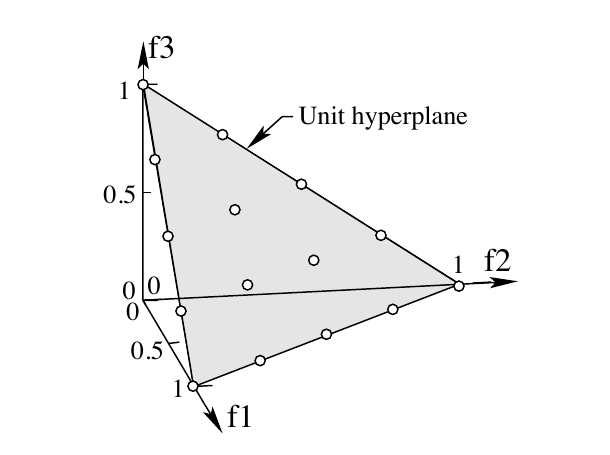
\includegraphics[scale=0.35]{hyper.png}
\caption{Hiperplano unitario generado con el método de Das \& Dennis}.
\end{figure}
Con los puntos de referencia y las magnitudes de las funciones objetivo normalizadas, se calcula la distancia ortogonal entre cada punto en nivel $l$ y se asocia a su punto de referencia más cercano,
seguido de un conteo de nichos para seleccionar a los miembros del nivel $l$ en los nichos menos poblados. Esto se repite hasta cumplir el criterio de paro.


\subsubsection{Pseudocódigo NSGA-III}
 
   \scalebox{.85}{
   \begin{algorithm}[H]
   \caption{Algoritmo NSGA-III}
     
 \KwData{$H$:puntos de referencia estructurados $\bm{Z}^{(s)}$, Población Padre $P_t$}
 \KwResult{$P_{t+1}$}
   $S_t=\emptyset,i=1$\;
   $Q_t = Recombinacion+Mutacion(P_t)$\;
   $R_t = P_t \cup Q_t$\;
   ($F_1,F_2,\dots$) = FastNondominatedSort($R_t$)\;
   
   \Repeat{$|S_t| \geq N$}{
   $S_t = S_t \cup F_i$\;
   $i=i+1$\;
   }
   $F_l = F_i$\;
   \eIf{$|S_t| == N$}{
   $P_{t+1} = S_t$\;
   break\;
   }(\tcc*[f]{Eleccion de los $K$ puntos restantes de $F_l$}){
   $P_{t+1}= \bigcup^{l-1}_{j=1} F_j$\;
   $K=N-\|P_{t+1}\|$\;
   $Normalizar(f^n,S_t,Z^r,Z^s,Z^a)$\;
   $(\pi(s),d(s))=Asociar(S_t,Z^r)$\;
   \For{$j \in Z^r$}{
   $\rho_j =\sum_{s \in S_t \setminus f_l } ( \pi(s) == j )$\;
    }
    $P_{t+1} = Nichos(K,\rho_j,\pi,d,Z^r,F_l, P_{t+1})$\;
   }
   
  \Return ($P_{t+1}$)
\end{algorithm}}


\subsection{Métodos empleados para resolver el MOP mejorando la diversidad de las soluciones}

Se han realizado varios esfuerzos enfocados a la mejora de la diversidad con ambas estrategias (descomposición con el \emph{MOEA/D} y dominancia con el \emph{NSGA-III}), la determinación de los vectores de peso o puntos de referencia constituye claramente un factor crítico para obtener una buena diversidad del frente aproximado. Se han propuesto varios algoritmos para generar vectores de pesos iniciales en el caso del enfoque de descomposición como:
\newline
% 
% \begin{itemize}
%  \item B. Liu et al. (2010) utilizan una variante de MOEA/D que sustituye al algoritmo genético por evolución diferencial (DE/best/1/bin). Los autores buscan mejorar la diversidad usando un factor de escalamiento aleatorio en la evolución diferencial, además de restringir la cruza al permitir aleatoriamente la reproducción de individuos fuera de la vecindad. Utilizan descomposición por el método de Tchebycheff \cite{5585957}.
%  \item T. C. Chiang \& Y. P. Lai (2011) consideran dos cambios fundamentales en la estructura de MOEA/D y MOEA/D-DE (en el que la generación de nuevas soluciones candidatas se realiza mediante el operador de mutación de Evolución Diferencial), el primero consiste en crear un criterio de selección del subproblema a resolver si es que éste no se considera resuelto (sin mejora tras cierto número de iteraciones) con el fin de redistribuir el tiempo de cómputo solo en los problemas aún sin resolver. La segunda mejora es la restricción a la cruza aplicada a los individuos en el espacio de las variables de decisión en lugar del espacio de los objetivos. Sin embargo, la generación de los nichos requiere ajustar dos parámetros adicionales que empeoran un proceso de agrupamiento computacionalmente costoso $O(nN^2)$\cite{5949789}.
%  \item S. Z. Zhao et al. (2010) proponen calcular el tamaño de vecindario en MOEA/D de forma dinámica, generando un ranking de los tamaños que estadísticamente dan mejores resultados. Este proceso se repite recalcula cada cierto número de generaciones, siendo entonces el tamaño de vecindario auto-adaptativo \cite{6151117}.
%  \item Haitham Seada \& Kalyanmoy Deb (2015) proponen un algoritmo basado en NSGA-III capaz de adaptarse y funcionar bien en problemas multiobjetivo, mono objetivo y de muchos objetivos ajustando los parámetros del algoritmo según la dimensión \cite{a0ecee762d9f4867a9ded8de598c732e}.
%  \item Giagkiozis et al. (2014) introducen el método Cross-entropy (CE) basado en métodos probabilísticos que distribuyen los puntos de referencia acorde a la geometría del frente de Pareto, de tal manera que se maximice el indicador de hipervolumen. CE utiliza métodos poblacionales y reacciona ante eventos para ajustar la distribución de probabilidad y adaptarse al frente \cite{Giagkiozis2014363}.
%  \item Haitham Seada \& Kalyanmoy Deb (2015) realizan un estudio sobre la restricción del tamaño de población impuesto en el NSGA-III original y proponen una aproximación que solventa esa deficiencia aprovechando las técnicas de nichos \cite{7257251}.
%  \end{itemize}



\begin{itemize}
 \item Cheng He \& Linquiang Pan (2016) proponen un método de generación de puntos tomando en cuenta las propiedades de la función objetivo y determinando si la superficie del frente es cóncava, convexa o un hiperplano. Este procedimiento se repite para numerosas subregiones del espacio objetivo, generando experimentalmente un conjunto de puntos mejor distribuidos (de acuerdo a la métrica de ``Espaciamiento'') que el método de referencia propuesto por Das y Dennis \cite{7748353}.    
 \item Das \& Dennis (1998) proponen utilizar ``Simplex Lattice'' para la generación de puntos de referencia iniciales en la optimización multiobjetivo \cite{Das:1998:NIN:588907.589322}, esta técnica proviene del diseño de mezclas y es ampliamente usada en los algoritmos evolutivos multiobjetivo \cite{4358754,6600851}.
 \item Zhang \& Deb (2015) introducen una técnica que amplía ``Simplex Lattice'' utilizando un modelo de dos capas que permite integrar puntos adicionales en una capa interna, evitando que en altas dimensiones la mayoría de los puntos queden cercanos a las fronteras del simplejo generado \cite{li2015evolutionary}.
 \item Tan \& Yan (2013) adaptan la técnica de diseño uniforme \cite{fang2000uniform} a la optimización multiobjetivo donde los puntos iniciales son la solución a un problema de optimización combinatoria que minimiza la métrica de discrepancia centrada $L_2$ \cite{tan2013moea,fang2002centered}.
 \item Zapotecas et al. (2015) proponen utilizar secuencias bien conocidas por generar un muestreo de baja discrepancia con la métrica $L_2$ simple, sin embargo, el costo computacional de generar los vectores de peso es $O(N \cdot k \cdot log k)$ \cite{zapotecas2015low}.
\end{itemize}

Cabe mencionar que las estrategias antes mencionadas fueron implementadas en un contexto de vectores/puntos de referencia estáticos a lo largo del proceso de búsqueda. Por otro lado, un área poco estudiada propone modificar los puntos/vectores de referencia de forma dinámica durante el transcurso del algoritmo de tal manera que éstos se ajusten a la geometría del $\mathcal{PF}_{true}$:
\begin{itemize}
  \item Jiang et al. (2011) proponen un parámetro $l$ que calibra la generación subproblemas lineales que maximizan el hipervolumen en una región, estos son resueltos con el método simplex, de tal manera que los vectores resultantes modelan la convexidad de la región \cite{jiang2011multiobjective}.
  \item Hi et al. (2011) introducen una preselección de vectores de peso de un conjunto $\sigma$  generado con simplex lattice. Estos vectores de peso son reevaluados con respecto  a la distancia euclidiana  a la solución no dominada más cercana y en su caso reemplazados por algún vector en $\sigma$ más cercano a dicha solución \cite{li2011adaptive}.
  \item Himanshu Jain \& Kalyanmoy Deb (2013) desarrollan una distribución adaptativa de los puntos de referencia para asegurar la diversidad, reubicando los puntos referencia que no han sido asociados a soluciones factibles hacia posiciones vecinas donde se espera tengan soluciones asociadas \cite{jain2013improved}.
  \item Yutao Qi et al. (2014) proponen modificar los vectores de peso conforme a esta estrategia permite generar medidas de dispersión promoviendo la generación de vectores adicionales en regiones con alta dispersión o, al contrario, la eliminación de ciertos vectores de regiones densamente pobladas \cite{doi:10.1162/EVCOa00109}.
  \item Yutao Qi et al. (2014) , basándose en su trabajo anterior, redefinen el vecindario en términos de triangulación de Delaunay como alternativa a los $k$ vecinos más cercanos, de tal manera que los triángulos tiendan a ser equiláteros separando y modificando los vectores de pesos en el transcurso del algoritmo \cite{qi2014moea}.
\end{itemize}

Como antes mencionado, esta última área ha sido poco explorada y el presente trabajo se propone el desarrollo de una estrategia para ajustar dinámicamente los vectores/puntos de referencia. Por ejemplo, una línea de investigación podría ser la adaptación de las ideas de repulsión de subpoblaciones, introducidas en la subsección siguiente.
\subsection{Repulsión de subpoblaciones}

En 2016, Ahrari et al. proponen utilizar una técnica de nichos basada en la repulsión de subpoblaciones \cite{ahrari2016multimodal}. Toda subpoblación $P_i$ tiene un tamaño fijo $\lambda$,
sus propios parámetros de cruza y mutación ($\sigma_{mean_i},C_i$), un centro ($x_{mean_i}$) y miembros élite. Existe también un conjunto de puntos prohibidos $y_k$
(mejores soluciones actuales o los centros de las subpoblaciones) que restringen la generación de nuevas soluciones en base a una métrica, de forma que las nuevas soluciones aceptables
se encontrarán en regiones poco exploradas del espacio de búsqueda. Una solución se considera aceptable si satisface el criterio distancia con todos los puntos prohibidos, de lo contrario,
la solución es rechazada. El efecto general de esta estrategia es una remodelación de las soluciones alcanzadas de tal manera que las subpoblaciones exploran en regiones del espacio
aún no visitadas previamente y prohibiendo que dos subpoblaciones busquen en la misma región del espacio de búsqueda.
\newline

Esta estrategia de nichos utiliza la distancia de Mahalanobis\cite{mahalanobis1936generalised}, una versión escalada de la distancia euclidiana, permitiendo revisar si una solución está lo suficientemente
alejada de los puntos prohibidos. La distancia de Mahalanobis ($D_{ij-k}$) de la $j$-ésima solución ($x_{ij}$) de $P_i$, matriz de covarianza $C_i$ y desviación estándar $\sigma_{mean_i}$ al punto prohibido
$y_k$, se define como sigue:

$$D_{ij-k} = \frac{(x_{ij}-y_k)^T C^{-1}_i (x_{ij}-y_k)}{\sigma_{mean_i}}$$

Una consecuencia del uso de esta distancia en particular es que $D_{ij-k}$ es inversamente proporcional a $\sigma_{mean_i}$, es decir, cuando las soluciones convergen $x_{ij}$ a $y_k$,
la distancia $D_{ij-k}$ aumenta. Este comportamiento evita que las nuevas soluciones sean similares a $y_k$.



\section{Justificación}

Las metaheurísticas son técnicas de solución versátiles, flexibles y eficientes, estos algoritmos pueden resolver problemas complejos de optimización multiobjetivo \cite{coello1999comprehensive} aproximando el frente real con éxito. 
De esta forma proporcionan un marco de trabajo accesible computacionalmente para encontrar soluciones de buena calidad que además sean diversas, permitiendo al tomador de decisiones efectuar la elección conforme a los criterios que le parezcan pertinentes.
\newline

Actualmente hay varios trabajos enfocados a mejorar las distribución de pesos. A pesar de que han tenido resultados prometedores \cite{4358754,6600851,li2015evolutionary,fang2000uniform}, aún es difícil conseguir una buena distribución en problemas
con frentes desconectados, frentes convexos y no convexos, con distribución no uniforme, etc. Problemas de aplicación suelen mostrar este tipo de características se encuentran en campos como:

\begin{itemize}
 \item Ingeniería automotriz \cite{6600851,liao2008multiobjective}.
 \item Ingeniería aeroespacial \cite{keskin2006application}.
 \item Mecatrónica \cite{affi2007advanced}.
 \item Energías renovables \cite{you2012optimal}.
\end{itemize}
 
El presente trabajo adquiere importancia con el estudio de los mecanismos que buscan preservar la diversidad de las soluciones en los principales marcos de trabajo en el estado del arte de \textbf{MOP}. En particular,
la inicialización de vectores de pesos/puntos de referencia iniciales y la capacidad de adaptar los mismos durante el transcurso de la ejecución de los algoritmos son vitales para alcanzar los objetivos de diversidad y convergencia. 
Tomando, por ejemplo, como referencia la técnica de repulsión de subpoblaciones proveniente de la optimización multimodal \cite{ahrari2016multimodal}, se propone introducir un método de adaptación de puntos de referencia/vectores de pesos que aproveche la información adquirida para redistribuir las referencias, y así mejorar la diversidad con respecto a alguna métrica.

\section{Objetivo General}

Adaptar e integrar estrategias de generación y actualización de los vectores de peso en el MOEA/D y de los puntos de referencia en el NSGA-III, para  evaluar su impacto sobre el desempeño en términos de diversidad de estos dos algoritmos evolutivos multiobjetivo.

\section{Objetivos Particulares}

\begin{itemize}

\item Adaptar, implementar y describir el comportamiento del método \emph{MOEA/D} para las instancias seleccionadas.
 
\item Adaptar, implementar y describir el comportamiento del método \emph{NSGA-III} para las instancias seleccionadas.

\item Adaptar e implementar al menos dos estrategias para generar vectores de peso /puntos de referencia iniciales para \emph{MOEA/D} y \emph{NSGA-III}.

\item Desarrollar al menos una estrategia de actualización de vectores de pesos para el método \emph{MOEA/D}, basada en el método de repulsión de subpoblacione \cite{ahrari2016multimodal}.

\item Desarrollar al menos una estrategia de actualización de puntos de referencia para el método \emph{NSGA-III}, basada en el método de repulsión de subpoblaciones \cite{ahrari2016multimodal}.
  
\item Realizar experimentos computacionales sobre un banco de instancias clásicas de optimización multiobjetivo \cite{zhang2008multiobjective} para comparar las diferentes versiones de los algoritmos estudiados, particularmente con respecto a las métricas de diversidad.

\item Realizar experimentos computacionales sobre un banco de instancias clásicas de optimización multiobjetivo \cite{zhang2008multiobjective} para comparar los resultados obtenidos con los reportados en la literatura especializada.  

\end{itemize}


\section{Metodología}

Para la implementación de las dos heurísticas basadas en los enfoques de descomposición y dominancia, se hizo una revisión en el estado del arte para analizar las características de los marcos de trabajo NSGA-III y MOEA/D, tomándolas  como  base para la adaptación al problema. Posteriormente se propondrán mejoras a estos algoritmos, como se describe a continuación.
\newline

Particularmente, se realizará un análisis estadístico de cada una de las técnicas implementadas, comparando su rendimiento contra algunas de las  técnicas propuestas en la literatura.
 
 \begin{itemize}
 \item[•] \textbf{ETAPA 1.} \emph{Se analizó el estado del arte para el MOEA/D y NSGA-III identificando los aportes recientes en cuestiones de diversidad.}
\item[] Se identificaron y listaron las técnicas reportadas en dos clases: métodos basados en descomposición y métodos basados en dominancia. Asimismo, se han revisado las técnicas enfocadas en la generación y actualización de los vectores de peso o puntos de referencia, de acuerdo a la clase de resolución utilizada.
\emph{(Concluida)}

\item[•] \textbf{Etapa 2.} \emph{Adaptación e implementación de los marcos de trabajo MOEA/D y NSGA-III, incluyendo, para cada uno, al menos dos técnicas de generación de vectores/puntos de referencia iniciales.}

\item[] Con base al análisis del perfil de nuestras técnicas, se implementarán en un lenguaje de programación.
        
\item[•] \textbf{Etapa 3.} \emph{Comparaciones de las técnicas y análisis estadístico.}

\item [] Una vez que se tengan las estrategias implementadas, se realizarán experimentos computacionales sobre bancos de problemas clásicamente utilizados en la literatura, como por ejemplo: la suite DTLZ, la suite WFG o la suite UF (CEC'2009) \cite{coello2007evolutionary,zhang2008multiobjective}. Así, se podrán efectuar comparaciones sobre la calidad de las soluciones obtenidas por cada versión de los dos marcos de trabajo estudiados, así como de la cantidad de recursos computacionales utilizados. Posteriormente, se justificará su rendimiento con un análisis estadístico detallado para cada versión implementada de los métodos de interés.

\item[•] \textbf{Etapa 4.} \emph{Proceso de mejora de las técnicas mediante la adaptación dinámica de los vectores/puntos de referencia.}

\item[] Se desarrollará una estrategia para actualizar los vectores/puntos de referencia, basada en la técnica de repulsión de subpoblaciones descrita en la sección [3.4].

\item[•] \textbf{Etapa 5.} \emph{Comparación de las técnicas definidas y reporte de resultados.}

\item[] Una vez terminada la etapa de mejoras de cada una de las técnicas, se realizará un nuevo análisis estadístico para comparar el rendimiento de cada una de nuestra técnicas, describiendo los resultados obtenidos.
        
\end{itemize}

         
\section{Cronograma}
\begin{table}[H]
\centering

\label{tablaTiempos}
\scalebox{0.7}{\begin{tabular}{|l|c|c|c|c|}
\hline
\begin{tabular}[c]{@{}c@{}}Nombre\\   de la tarea\end{tabular} & Trimestre & Semanas & Duración \\ \hline
Implementación de al menos dos técnicas de generación de los vectores de peso/puntos de referencia& 18I        & 1-3   & 3 semanas     \\ \hline
Implementación de la técnica MOEA/D y pruebas preliminares     & 18I       & 4-6    & 3 semanas     \\ \hline
Implementación de la técnica NSGA-III y pruebas preliminares   & 18I        & 7-9    & 3 semanas      \\ \hline
Diseño de una estrategia de actualización de los vectores de peso/puntos de referencia basada en \cite{ahrari2016multimodal} & 18I        & 10-11    &    2 semanas      \\ \hline
Adaptación e implementación de la estrategia de actualización en NSGA-III y MOEA/D & 18P        & 1-4    &   4 semanas      \\ \hline
Experimentos computacionales definitivos, análisis y comparación de técnicas  & 18P        & 5-8       & 4 semanas      \\ \hline
Redacción de tesis                                             & 18P        &  5-11   &    7 semanas     \\ \hline
\end{tabular}
}
\caption{Cronograma}
\end{table}



% \begin{table}[H]
% \centering
% \label{miOtraTabla}
% \scalebox{0.6}{\begin{tabular}{|l|l|}
% \hline
% Nombre de la tarea                 & \multicolumn{1}{c|}{Metas alcanzar al terminar la tarea}                                                                                                                                                                                                                                                                                                                                                            \\ \hline
% Presentación propuesta de tesis    & Aprobación de propuesta de tesis por el comité de posgrado.                                                                                                                                                                                                                                                                                                                                                         \\ \hline
% Correcciones propuesta de tesis    & Registro de Aceptación de tesis.                                                                                                                                                                                                                                                                                                                                                                                    \\ \hline
% Adaptación FA para el PAG          & \begin{tabular}[c]{@{}l@{}}Se busca describir el comportamiento de la técnica implementada al PAG y probada\\ con algunas instancias disponibles, esperando tener buenos resultados con respecto de\\  las técnicas existentes en la literatura,  comparando la calidad de la solución y el número\\  de llamadas a la función objetivo;  así como las ventajas y desventajas que ofrece esta técnica.\end{tabular} \\ \hline
% Adaptación GSA para el PAG         & \begin{tabular}[c]{@{}l@{}}Se busca describir el comportamiento de la técnica implementada al PAG  y probada \\ con algunas instancias disponibles,  esperando tener buenos resultados con respecto de\\ las técnicas existentes en la literatura, comparando la calidad de la solución y el número\\ de llamadas a la función objetivo; así como las ventajas y desventajas que ofrece esta técnica.\end{tabular}  \\ \hline
% Adaptación MMC para el PAG         & \begin{tabular}[c]{@{}l@{}}Se busca describir el comportamiento de la técnica implementada al PAG y probada \\ con algunas instancias disponibles, esperando tener buenos resultados con respecto de \\ las técnicas existentes en la literatura, comparando la calidad de la solución y el número\\ de llamadas a la función objetivo;  así como las ventajas y desventajas que ofrece esta técnica.\end{tabular}  \\ \hline
% Anélisis y comparación de técnicas & \begin{tabular}[c]{@{}l@{}}Se busca describir el comportamiento de nuestras técnicas con la finalidad de poder\\ decir cuales son sus ventajas o defectos al ser utilizadas con las instancias seleccionadas\\ para el PAG.\end{tabular}                                                                                                                                                                            \\ \hline
% Redacción de tesis                 & Documentación de la investigación realizada.                                                                                                                                                                                                                                                                                                                                                                        \\ \hline
% Entrega de tesis                   & \begin{tabular}[c]{@{}l@{}}Obtener la\\   aprobación y fecha para el examen de grado\end{tabular}                                                                                                                                                                                                                                                                                                                   \\ \hline
% \end{tabular}
% }
% \caption{Metas}
% \end{table}

%\begin{figure}[H]
%\begin{center}
    %\scalebox{0.800}{\includegraphics{cronogramatesis.jpg}}%%%%%%%%%%%%%%%%%%Cambiar imagen.
 
 % \label{sol}
%   \caption{Cronograma.}
   
%\end{center}
%\end{figure}

%\begin{figure}[H]
%\begin{center}
%    \scalebox{0.600}{\includegraphics{cronograma2.jpg}}%%%%%%%%%%%%%%%%%%Cambiar imagen.
 
 % \label{sol}
  % \caption{Cronograma2.}
   
%\end{center}
%\end{figure}
\bibliographystyle{acm}
\bibliography{bibliografia}
\end{document}